\chapter{Bảng trạng thái đầy đủ các máy trạng thái}
\label{app:fsm}

Phụ lục này liệt kê đầy đủ các trạng thái của mọi máy trạng thái trong lõi giao thức, bổ trợ cho
\cref{ch:architecture}. Tên trạng thái giữ nguyên định danh RTL.

\section*{\SclGenerator{} — \SclStateCount{} trạng thái}

\begin{longtable}{C{1.2cm} L{4.2cm} L{7.2cm}}
	\toprule
	\textbf{\#} & \textbf{Trạng thái}       & \textbf{Vai trò}                                \\
	\midrule\endhead
	0           & \texttt{Idle}             & Chờ yêu cầu phát START/xung nhịp.               \\
	1           & \texttt{GenerateStart}    & Bắt đầu tạo điều kiện START.                    \\
	2           & \texttt{SdaFall}          & Kéo SDA xuống khi SCL cao để tạo START hoặc \RepeatedSTART{}. \\
	3           & \texttt{HoldStart}        & Giữ điều kiện START.                            \\
	4           & \texttt{DriveLow}         & Kéo SCL xuống (nửa chu kỳ thấp).                \\
	5           & \texttt{DriveHigh}        & Thả SCL lên (nửa chu kỳ cao).                   \\
	6           & \texttt{WaitCmd}          & Chờ lệnh/dữ liệu tiếp theo giữa chừng.          \\
	7           & \texttt{GenerateRstart}   & Bắt đầu tạo \RepeatedSTART{}.                   \\
	8           & \texttt{SclHighForRstart} & Đưa SCL lên để chuẩn bị \RepeatedSTART{}.       \\
	9           & \texttt{GenerateStop}     & Bắt đầu tạo điều kiện STOP.                     \\
	10          & \texttt{SclHighForStop}   & Đưa SCL lên để chuẩn bị STOP.                   \\
	11          & \texttt{SdaRise}          & Thả SDA lên khi SCL cao (STOP).                 \\
	12          & \texttt{BusFree}          & Đợi \BusFreeCondition{} sau STOP.               \\
	\bottomrule
\end{longtable}

\begin{figure}[!htbp]
	\centering
	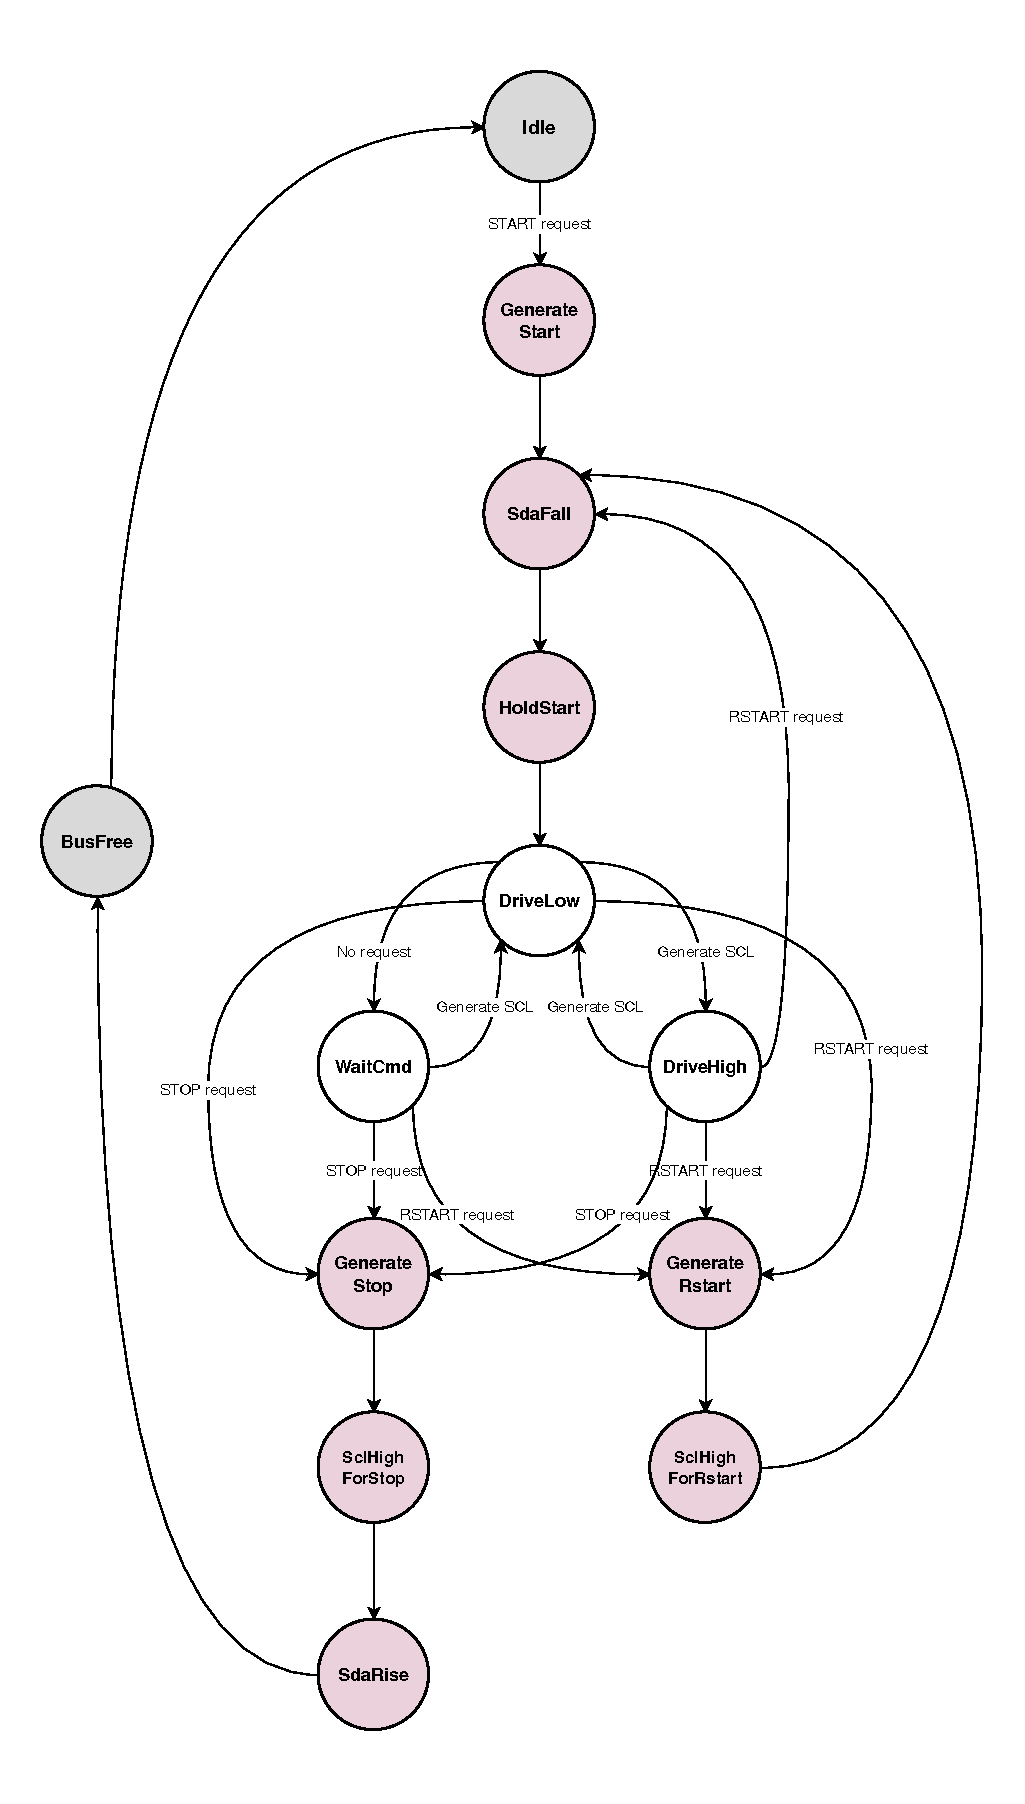
\includegraphics[width=\textwidth,height=0.72\textheight,keepaspectratio]{figures/scl_generator_fsm.pdf}
	\caption{Sơ đồ chuyển trạng thái của \SclGenerator{}.}
	\label{fig:scl-gen-fsm}
\end{figure}

\section*{\EntdaaController{} — \EntdaaControllerStateCount{} trạng thái}

\begin{longtable}{C{1.2cm} L{4.2cm} L{7.2cm}}
	\toprule
	\textbf{\#} & \textbf{Trạng thái}    & \textbf{Vai trò}                           \\
	\midrule\endhead
	0           & \texttt{Idle}          & Chờ khởi động ENTDAA.                      \\
	1           & \texttt{StartLoop}     & Bắt đầu một vòng gán địa chỉ.              \\
	2           & \texttt{RequestRStart} & Yêu cầu \RepeatedSTART{}.                  \\
	3           & \texttt{WaitRStart}    & Chờ \RepeatedSTART{} hoàn tất.             \\
	4           & \texttt{ReadDAT}       & Đọc mục DAT lấy \DynamicAddress{} cần cấp. \\
	5           & \texttt{RunEntdaa}     & Chạy một vòng gán qua \EntdaaFsm{}.        \\
	6           & \texttt{Done}          & Kết thúc khi không còn \Target{} đáp ứng.  \\
	\bottomrule
\end{longtable}

\begin{figure}[!htbp]
	\centering
	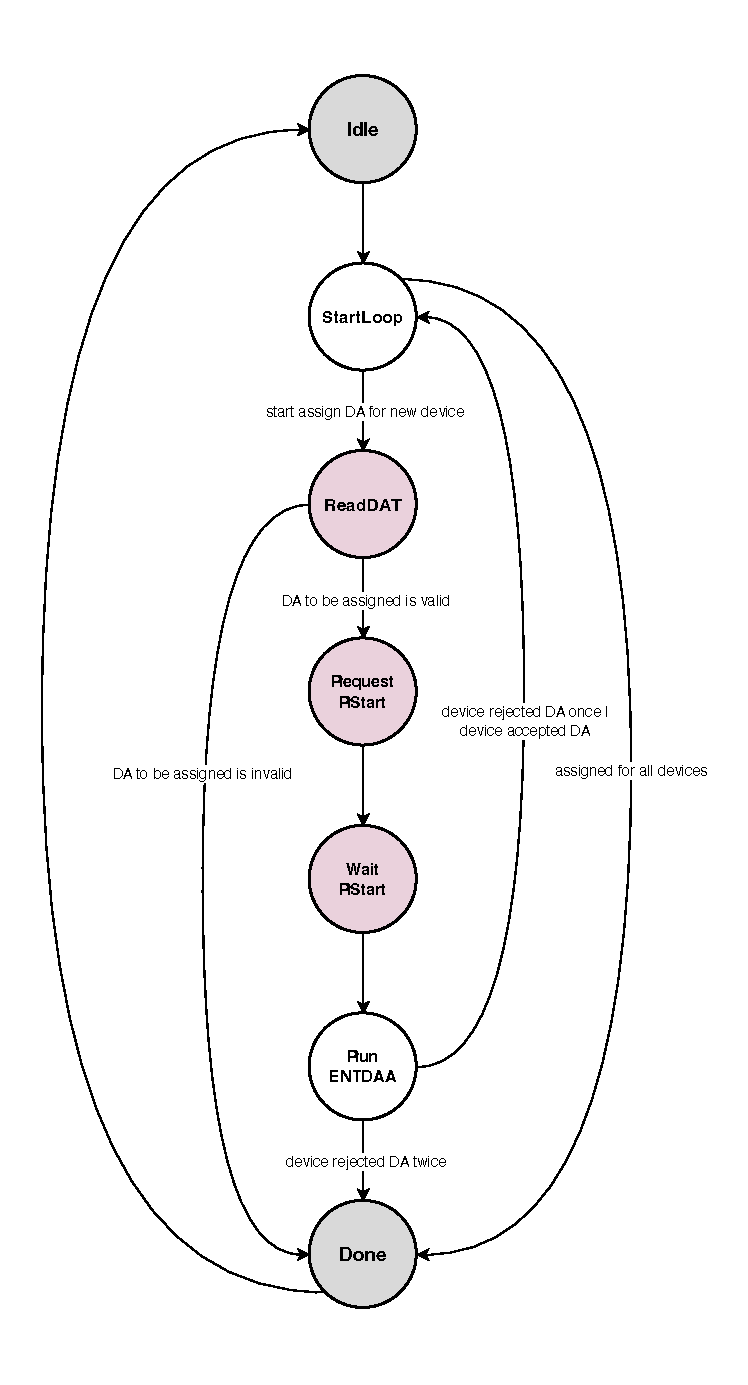
\includegraphics[width=\textwidth,height=0.72\textheight,keepaspectratio]{figures/entdaa_controller_fsm.pdf}
	\caption{Sơ đồ chuyển trạng thái của \EntdaaController{}.}
	\label{fig:entdaa-controller-fsm}
\end{figure}

\section*{\EntdaaFsm{} — \EntdaaFsmStateCount{} trạng thái}

\begin{longtable}{C{1.2cm} L{4.2cm} L{7.2cm}}
	\toprule
	\textbf{\#} & \textbf{Trạng thái}       & \textbf{Vai trò}                                    \\
	\midrule\endhead
	0           & \texttt{Idle}             & Chờ bắt đầu trình tự một \Target{}.                 \\
	1           & \texttt{SendDAAHeader}    & Phát \IThreeCBroadcastAddress{} dành riêng.          \\
	2           & \texttt{ReceiveHeaderACK} & Đọc ACK của byte dành riêng.                        \\
	3           & \texttt{ReceiveID}        & Nhận 64 bit PID/BCR/DCR theo phân xử.               \\
	4           & \texttt{SendDynamicAddr}  & Phát \DynamicAddress{} kèm parity.                  \\
	5           & \texttt{ReceiveAddrACK}   & Đọc ACK địa chỉ từ \Target{}.                       \\
	6           & \texttt{WaitStop}         & Chờ điều kiện dừng.                                 \\
	7           & \texttt{Done}             & Hoàn tất một vòng.                                  \\
	\bottomrule
\end{longtable}

\begin{figure}[!htbp]
	\centering
	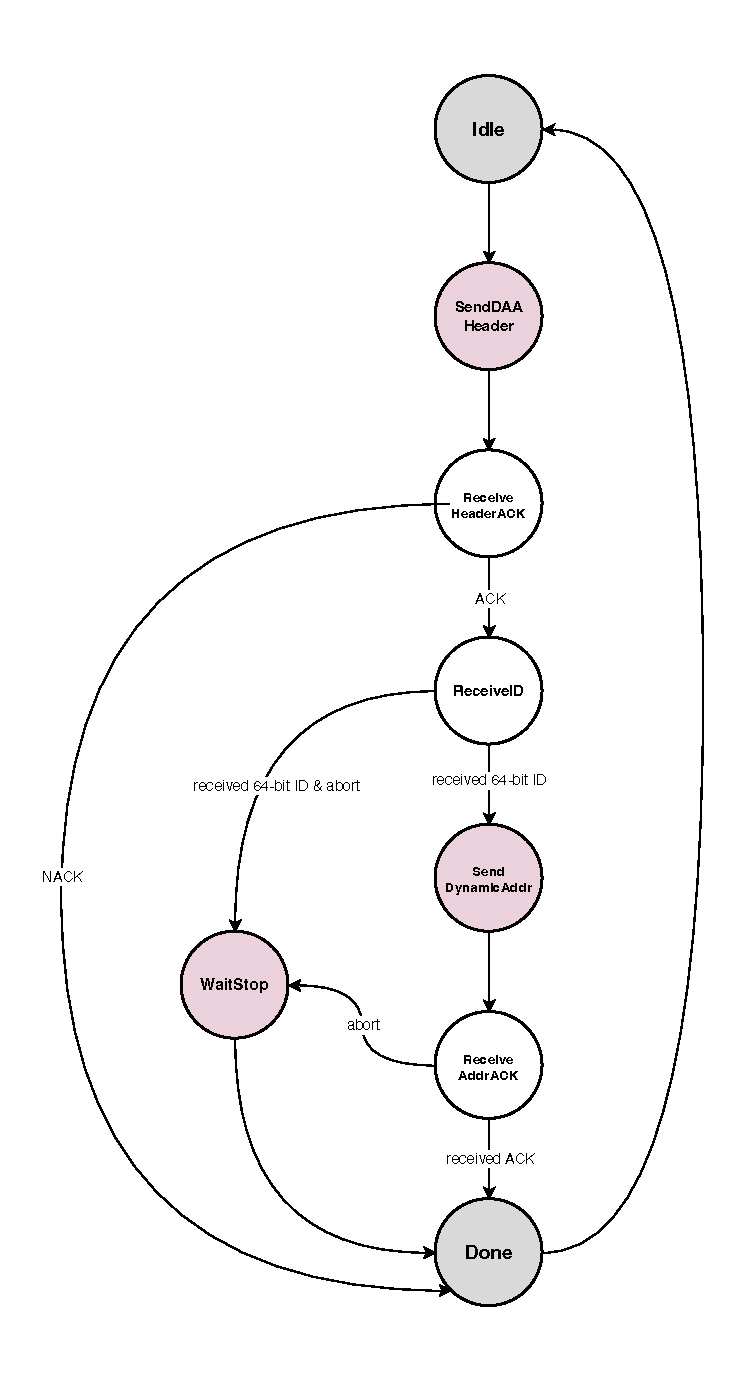
\includegraphics[width=\textwidth,height=0.72\textheight,keepaspectratio]{figures/entdaa_fsm.pdf}
	\caption{Sơ đồ chuyển trạng thái của \EntdaaFsm{}.}
	\label{fig:entdaa-fsm}
\end{figure}

\section*{Các máy trạng thái tuần tự hóa}

\subsection*{\BusTx{} — \BusTxStateCount{} trạng thái}

\begin{longtable}{C{1.2cm} L{4.2cm} L{7.2cm}}
	\toprule
	\textbf{\#} & \textbf{Trạng thái}        & \textbf{Vai trò}                                        \\
	\midrule\endhead
	0           & \texttt{Idle}              & Chờ yêu cầu phát một bit hoặc một byte.                 \\
	1           & \texttt{AwaitClockNegedge} & Chờ cạnh xuống SCL để canh thời điểm đặt dữ liệu.       \\
	2           & \texttt{SetupData}         & Giữ khoảng setup dữ liệu trước khi phát bit.            \\
	3           & \texttt{TransmitData}      & Lái bit dữ liệu ra SDA trong nửa chu kỳ SCL.            \\
	4           & \texttt{HoldData}          & Giữ khoảng hold sau bit trước khi trở về \texttt{Idle}. \\
	\bottomrule
\end{longtable}

\subsection*{\BusTxFlow{} — \BusTxFlowStateCount{} trạng thái}

\begin{longtable}{C{1.2cm} L{4.2cm} L{7.2cm}}
	\toprule
	\textbf{\#} & \textbf{Trạng thái}       & \textbf{Vai trò}                                            \\
	\midrule\endhead
	0           & \texttt{Idle}             & Chờ yêu cầu phát byte hoặc bit.                             \\
	1           & \texttt{DriveByte}        & Điều phối phát lần lượt 8 bit của một byte qua \BusTx{}.    \\
	2           & \texttt{DriveBit}         & Điều phối phát một bit đơn (ACK hoặc \TBit{}) qua \BusTx{}. \\
	3           & \texttt{NextTaskDecision} & Quyết định phát byte/bit kế tiếp hay trở về \texttt{Idle}.  \\
	\bottomrule
\end{longtable}

\subsection*{\BusRxFlow{} — \BusRxFlowStateCount{} trạng thái}

\begin{longtable}{C{1.2cm} L{4.2cm} L{7.2cm}}
	\toprule
	\textbf{\#} & \textbf{Trạng thái}       & \textbf{Vai trò}                                           \\
	\midrule\endhead
	0           & \texttt{Idle}             & Chờ yêu cầu nhận byte hoặc bit.                            \\
	1           & \texttt{ReadByte}         & Điều phối nhận lần lượt 8 bit của một byte.                \\
	2           & \texttt{ReadBit}          & Điều phối nhận một bit đơn (ACK hoặc \TBit{}).             \\
	3           & \texttt{NextTaskDecision} & Quyết định nhận byte/bit kế tiếp hay trở về \texttt{Idle}. \\
	\bottomrule
\end{longtable}

\section*{\FlowActive{} — \FlowStateCount{} trạng thái}

\noindent Luồng điều khiển trung tâm được trình bày ở mức giao thức tại
\cref{sec:flow-states}. \Cref{tab:flow-states} liệt kê đầy đủ các trạng thái theo định danh RTL.

\begin{table}[!htbp]
	\centering
	\caption{Vai trò tóm tắt của \FlowStateCount{} trạng thái trong khối điều khiển trung tâm.}
	\label{tab:flow-states}
	\begin{tabular}{C{1.0cm} L{4.0cm} L{7.4cm}}
		\toprule
		\textbf{\#} & \textbf{Trạng thái}        & \textbf{Vai trò}                                                        \\
		\midrule
		0           & \texttt{Idle}              & Xóa context giao dịch, giữ bus ở trạng thái nghỉ.                       \\
		1           & \texttt{WaitForCmd}        & Chờ \CommandFifo{} cung cấp \CommandDescriptor{}.                       \\
		2           & \texttt{FetchDAT}          & Kiểm tra \CommandDescriptor{}, phát yêu cầu đọc DAT.                    \\
		3           & \texttt{WaitDAT}           & Chờ dữ liệu DAT, quyết định nhánh giao thức.                            \\
		4           & \texttt{I3CBcastHeader}    & Phát \IThreeCBroadcastAddress{} khi bit \texttt{IBA\_INCLUDE} được bật. \\
		5           & \texttt{IssueImmediateCcc} & Phát Broadcast/Direct ENEC hoặc DISEC.                                  \\
		6           & \texttt{FetchTxData}       & Lấy DWORD tiếp theo từ \TxFifo{}.                                       \\
		7           & \texttt{InitWrite}         & Phát \AddressHeader{} cho giao dịch ghi (I3C/\iic{}).                   \\
		8           & \texttt{InitRead}          & Phát \AddressHeader{} cho giao dịch đọc (I3C/\iic{}).                   \\
		9           & \texttt{IssueDAA}          & Chạy quy trình ENTDAA.                                                  \\
		10          & \texttt{IssueI3CWrite}     & Truyền dữ liệu I3C ghi, \TBit{}, continuation.                          \\
		11          & \texttt{IssueI2CWrite}     & Truyền dữ liệu \iic{} ghi, xác nhận ACK/NACK.                           \\
		12          & \texttt{IssueI3CRead}      & Nhận dữ liệu I3C đọc, giành lại quyền lái SDA sau \TBit{}, xử lý yêu cầu hủy giao dịch từ \Host{}. \\
		13          & \texttt{IssueI2CRead}      & Nhận dữ liệu \iic{} đọc, ACK/NACK, NACK-then-STOP.                      \\
		14          & \texttt{WriteResp}         & Ghi \ResponseDescriptor{}.                                             \\
		\bottomrule
	\end{tabular}
\end{table}
